\documentclass[
	handout,
%  	aspectratio=43
  	aspectratio=169
]{beamer}

\usepackage[utf8]{inputenc}
\usepackage[german]{babel}
\usepackage[figurename=Bild]{caption}
\usepackage{graphicx}
\usepackage{amsmath}
\usepackage{scrextend}
\usepackage{xcolor,colortbl}	
\usepackage{lmodern}	
\usepackage{amsmath,amssymb}
\usepackage{booktabs}

\title[Semesterprojekt KNIME]{Data Mining}

\date{18.06.2021}
\author[C. Werner, J. Prothmann]{C. Werner, J. Prothmann}


\institute{Bereich Elektrotechnik und Informatik}
\usetheme{Wismar}	% Design der Hochschule Wismar
\usecolortheme{FIW}

% Die Navigationshilfen unteren Folienrand kann man ausblenden
\beamertemplatenavigationsymbolsempty
% \beamertemplatefootempty

% Wenn mathematische Umgebungen in klassischer "Mathe-Schrift"
% dargestellt werden sollen, folgende Zeile entkommentieren.
%\usefonttheme[onlymath]{serif}

% Zeige Abschnittstitel auf separater Folie vor jedem Abschnitt
%\AtBeginSection{\frame{\sectionpage}}

\begin{document}
	\begin{frame}[plain]
		\titlepage
	\end{frame}

	\begin{frame}{Gliederung}
		\tableofcontents
	\end{frame}
		
\section{Vorverarbeitung}
\frame{\sectionpage}
\begin{frame}{Rohdatensatz}
\begin{figure}[!h]

	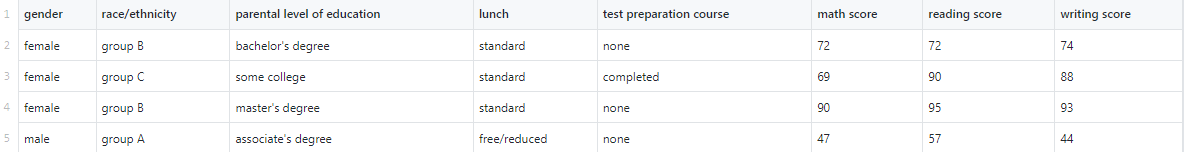
\includegraphics[scale= 0.55]{../pictures/roh.png}
	\caption{Rohdatensatz}
\end{figure}
\end{frame}
\begin{frame}{Datenvorverarbeitung}
\begin{figure}[!h]

	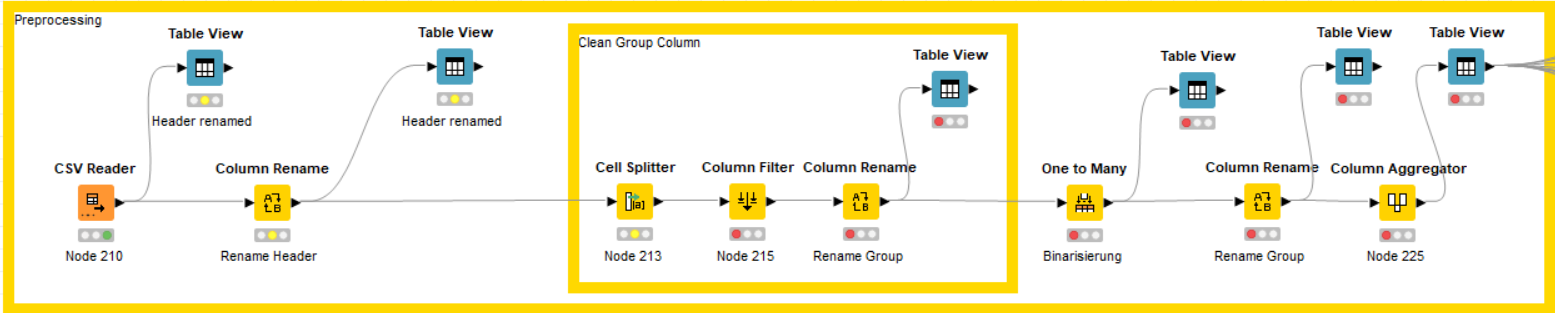
\includegraphics[scale= 0.45]{../pictures/preprocessing.png}
	\caption{Knime Workflow zur Vorverarbeitung}
\end{figure}
\end{frame}

\begin{frame}
\begin{figure}[!h]

	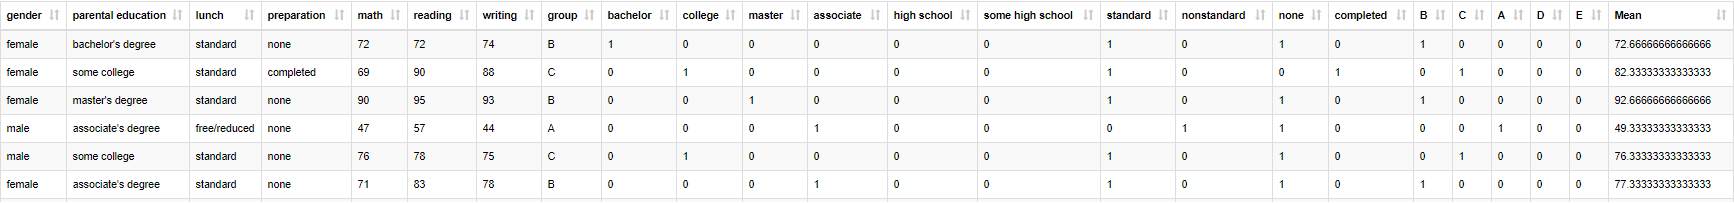
\includegraphics[scale= 0.4]{../pictures/processed.png}
	\caption{Vorverarbeitete Daten}
\end{figure}
\end{frame}

\section{Knime Knoten}
\frame{\sectionpage}
\end{document}
